%%%%%%%%%%%%%%%%%%%%%%%%%%%%%%%%%%%%%%%%%%%%%%%%%%%%%%%%%%%%%%%
%
% Welcome to Overleaf --- just edit your LaTeX on the left,
% and we'll compile it for you on the right. If you open the
% 'Share' menu, you can invite other users to edit at the same
% time. See www.overleaf.com/learn for more info. Enjoy!
%
%%%%%%%%%%%%%%%%%%%%%%%%%%%%%%%%%%%%%%%%%%%%%%%%%%%%%%%%%%%%%%%
% Author: Izaak Neutelings (June 2020)
% Inspiration: https://tex.stackexchange.com/questions/285578/how-to-draw-parallelepiped-and-cube-with-latex/288101#288101
\documentclass[border=3pt,tikz]{standalone}
\usepackage[outline]{contour} % glow around text
\usepackage{xcolor}
\usepackage{etoolbox} %ifthen
\usetikzlibrary{arrows,arrows.meta}
\usetikzlibrary{calc}
\usetikzlibrary{decorations.markings}
\usetikzlibrary{angles,quotes} % for pic (angle labels)
\tikzset{>=latex} % for LaTeX arrow head
\contourlength{1.6pt}

\colorlet{myblue}{blue!70!black}
\colorlet{myred}{red!65!black}
\colorlet{mypurple}{red!50!blue!95!black!75}
\colorlet{mylightgreen}{green!60!black!70}
\colorlet{mygreen}{green!60!black}
\colorlet{myredgrey}{red!50!black!80}
\tikzstyle{wave}=[myblue,thick]
\tikzstyle{mydashed}=[black!70,dashed,thin]
\tikzstyle{mymeas}=[{Latex[length=3,width=2]}-{Latex[length=3,width=2]},thin]



\begin{document}


% DESTRUCTIVE INTERFERENCE
\def\A{0.5}
\def\k{360}
\def\xmin{-0.3}
\def\xmax{4.4}
\def\h{2.3}
\def\lang{90}
\def\rang{270} % 720+270 = 990
\def\nsamples{200}
\begin{tikzpicture}
  %\def\angg{asin(\na/\ng*sin(\anga))}
  %\coordinate (O) at (0,0);
  
  % WAVE 1
  \draw[->,black]
    (\xmin,0) -- (1.06*\xmax,0);
  \draw[wave,variable=\x,samples=\nsamples,smooth,domain=\xmin:\xmax]
    plot(\x,{\A*sin(\k*\x)});
  \node at (\xmax/2,-\h/2) {$+$};
  
  % WAVE 2
  \begin{scope}[shift={(0,-\h)}]
    \draw[->,black]
      (\xmin,0) -- (1.06*\xmax,0);
    \draw[wave,myred,variable=\x,samples=\nsamples,smooth,variable=\x,domain=\xmin:\xmax]
      plot(\x,{\A*sin(\k*\x+180)});
  \end{scope}
  \node at (\xmax/2,-1.5*\h) {$=$};
  
  % WAVE 3
  \begin{scope}[shift={(0,-2*\h)}]
    \draw[->,black]
      (\xmin,0) -- (1.06*\xmax,0);
    \draw[wave,mypurple]
      (\xmin,0) -- (\xmax,0);
  \end{scope}
  
  % DASHED
  \draw[mydashed]
    (\lang/\k,1.25*\A) -- (\lang/\k,-2*\h-2.3*\A);
  \draw[mydashed]
    (\rang/\k,1.25*\A) -- (\rang/\k,-2*\h-2.3*\A);
  \draw[mymeas,myredgrey]
    (\lang/\k,-2.15*\A) --++ (180/\k,0)
    node[midway,below,scale=0.8] {\contour{white}{$\Delta \phi=\frac{\pi}{2}$}};
  
\end{tikzpicture}


% PARTIAL INTERFERENCE
\begin{tikzpicture}
  \def\dphi{138}
  
  % WAVE 1
  \draw[->,black]
    (\xmin,0) -- (1.06*\xmax,0);
  \draw[wave,variable=\x,samples=\nsamples,smooth,domain=\xmin:\xmax]
    plot(\x,{\A*sin(\k*\x)});
  \node at (\xmax/2,-\h/2) {$+$};
  
  % WAVE 2
  \begin{scope}[shift={(0,-\h)}]
    \draw[->,black]
      (\xmin,0) -- (1.06*\xmax,0);
    \draw[wave,myred,variable=\x,samples=\nsamples,smooth,domain=\xmin:\xmax]
      plot(\x,{\A*sin(\k*\x-\dphi)});
  \end{scope}
  \node at (\xmax/2,-1.5*\h) {$=$};
  
  % WAVE 3
  \begin{scope}[shift={(0,-2*\h)}]
    \draw[->,black]
      (\xmin,0) -- (1.06*\xmax,0);
    \draw[wave,mypurple,variable=\x,samples=\nsamples,smooth,domain=\xmin:\xmax]
      plot(\x,{2*cos(\dphi/2)*\A*sin(\k*\x-\dphi/2)});
  \end{scope}
  
  % DASHED
  \draw[mydashed]
    (\lang/\k,1.25*\A) -- (\lang/\k,-2*\h-2.3*\A);
  \draw[mydashed]
    (\rang/\k,1.25*\A) -- (\rang/\k,-2*\h-2.3*\A);
  \draw[mydashed,myredgrey]
    ({(\lang+\dphi)/\k},0.55*\A) -- ({(\lang+\dphi)/\k},-\h-1.3*\A);
  \draw[mymeas,myredgrey]
    (\lang/\k,-2.1*\A) --++ (\dphi/\k,0)
    node[midway,below,scale=0.8] {\contour{white}{$\Delta \phi$}};
  \draw[mymeas]
    (0.3*\xmin+\dphi/\k/2,-2*\h) --++ (0,{2*cos(\dphi/2)*\A})
    node[inner sep=-3,scale=0.8,below=4,left=4] %fill=white
      {$2A\cos\!\frac{\color{myredgrey}\Delta\phi}{2}$};
  
\end{tikzpicture}


% CONSTRUCTIVE INTERFERENCE
\begin{tikzpicture}
  
  % WAVE 1
  \draw[->,black]
    (\xmin,0) -- (1.06*\xmax,0);
  \draw[wave,variable=\x,samples=\nsamples,smooth,domain=\xmin:\xmax]
    plot(\x,{\A*sin(\k*\x)});
  \node at (\xmax/2,-\h/2) {$+$};
  
  % WAVE 2
  \begin{scope}[shift={(0,-\h)}]
    \draw[->,black]
      (\xmin,0) -- (1.06*\xmax,0);
    \draw[wave,myred,variable=\x,samples=\nsamples,smooth,domain=\xmin:\xmax]
      plot(\x,{\A*sin(\k*\x)});
  \end{scope}
  \node at (\xmax/2,-1.4*\h) {$=$};
  
  % WAVE 3
  \begin{scope}[shift={(0,-2*\h)}]
    \draw[->,black]
      (\xmin,0) -- (1.06*\xmax,0);
    \draw[wave,mypurple,variable=\x,samples=\nsamples,smooth,domain=\xmin:\xmax]
      plot(\x,{2*\A*sin(\k*\x)});
  \end{scope}
  
  % DASHED
  \draw[mydashed]
    (\lang/\k,1.25*\A) -- (\lang/\k,-2*\h-2.3*\A);
  \draw[mydashed]
    (\rang/\k,1.25*\A) -- (\rang/\k,-2*\h-2.3*\A);
  \draw[mymeas]
    (0.7*\xmin,-2*\h) --++ (0,2*\A)
    node[fill=white,midway,inner sep=1,scale=0.8] {$2A$};
  
\end{tikzpicture}


% POINT SOURCES
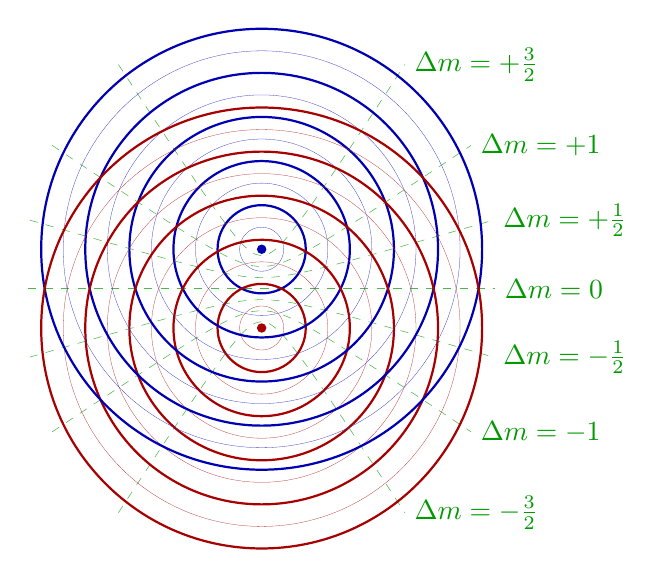
\begin{tikzpicture}[
    nodal/.style={mylightgreen,dashed,very thin},
    declare function={
      %xnode(\n,\dn,\lam,\f) = sqrt( (\n^2+(\n+\dn)^2)*\lambd^2/2 - (\n^2-(\n+\dn)^2)^2*\lambd^4/(4*\a^2) - \a^2/4 );
      xnode(\n,\dn,\lam,\f) = \lam/\f*sqrt( \n^2*(\f^2-\dn^2)+\n*\dn*(\f^2-\dn^2)+\dn^2*\f^2/2-(\f^4+\dn^4)/4 );
      ynode(\n,\dn,\lam,\a) = (2*\n*\dn+\dn^2)*\lam/(2*\f);
      intensity(\y,\lam,\a,\L) = cos(180*\a*\y/(2*\lam*sqrt(\L*\L+\y*\y)))^2;
    }
  ]
  
  %\def\W{2.2}
  %\def\H{2.2}
  \def\N{10}
  \def\lambd{0.28}
  \def\R{\N*\lambd}
  \def\a{1.0}
  \def\Nlines{3}
  \def\r{0.06}
  %\def\nmax{10}
  \def\nsamples{150}
  
  % NODAL LINES
  \draw[nodal]
    (-1.06*\R,0) -- (1.06*\R,0) node[mygreen,right] {$\Delta m=0$};
  % -1/2 + (1/0.44)/2 = 0.6363636364
  % -2/2 + (1/0.44)/2 = 0.1363636364
  % \c=int(\dn<int(\lambd))
  %\begin{scope}
    %\clip (-1.1*\W,-1.1*\H) rectangle (1.1*\W,1.1*\H);
    %\clip (0,0) ellipse ({1.1*\R} and {(1.1*(\R-\a/2)});
    %\clip (0,0) circle (1.1*\R);
  \foreach \dn [evaluate={
                 \f=\a/\lambd;
                 \nmin=0.501*(-\dn+\f);
                 \nmax=1.06*\N;
                 \meven=int(\dn-1);
                 \c=int(\dn<\f);}
               ] in {1,...,\Nlines}{
    \ifnum\c=1
      \draw[nodal,variable=\n,samples=\nsamples,smooth]
        plot[domain=\nmax:\nmin] ({-xnode(\n,\dn,\lambd,\f)},{ynode(\n,\dn,\lambd,\a)}) --
        plot[domain=\nmin:\nmax] ({xnode(\n,\dn,\lambd,\f)},{ynode(\n,\dn,\lambd,\a)})
        coordinate (+DN); %node[mygreen,right] {$\Delta m=\dn$};
      \draw[nodal,variable=\n,samples=\nsamples,smooth]
        plot[domain=\nmax:\nmin] ({-xnode(\n,\dn,\lambd,\f)},{-ynode(\n,\dn,\lambd,\a)}) --
        plot[domain=\nmin:\nmax] ({xnode(\n,\dn,\lambd,\f)},{-ynode(\n,\dn,\lambd,\a)})
        coordinate (-DN); %node[mygreen,right] {$\Delta m=-\dn$};
      \ifodd\dn
        \node[mygreen,right] at (-DN) {$\Delta m=-\frac{\dn}{2}$};
        \node[mygreen,right] at (+DN) {$\Delta m=+\frac{\dn}{2}$};
      \else
        \node[mygreen,right] at (-DN) {$\Delta m=-\meven$};
        \node[mygreen,right] at (+DN) {$\Delta m=+\meven$};
      \fi
    \fi
  }
  %\end{scope}
  
  % WAVES
  %\begin{scope}
    %\clip (-\W,-\H) rectangle (\W,\H);
  \foreach \i [evaluate={\R=\i*\lambd;}] in {1,...,\N}{
    \ifodd\i
      \draw[myblue!80,line width=0.1] (0,\a/2) circle (\R);
      \draw[myred!80,line width=0.1] (0,-\a/2) circle (\R);
    \else
      \draw[myblue,line width=0.8] (0,\a/2) circle (\R);
      \draw[myred,line width=0.8] (0,-\a/2) circle (\R);
    \fi
  }
  %\end{scope}
  
  % POINTS
  \fill[myblue] (0,\a/2) circle (\r); %node[left] {\contour{white}{S$_1$}};
  \fill[myred] (0,-\a/2) circle (\r); %node[left] {\contour{white}{S$_2$}};
  
\end{tikzpicture}


% PATH DIFFERENCE
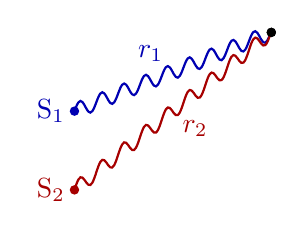
\begin{tikzpicture}
  
  \def\a{1}
  \def\px{2.5}
  \def\py{1.5}
  \def\A{0.1}
  \def\k{1300}
  \def\r{0.06}
  \coordinate (S1) at (0,\a/2);
  \coordinate (S2) at (0,-\a/2);
  \coordinate (P) at (\px,\py);
  
  % WAVES
  \draw[myblue,thick,samples=100,smooth,variable=\x,domain=0:1*\px]
    plot(\x,{\a/2+(\py-\a/2)/\px*\x + \A*sin(\k*\x)});
  \fill (\px,\py) circle (\r);
  \draw[myred,thick,samples=100,smooth,variable=\x,domain=0:1*\px]
    plot(\x,{-\a/2+(\py+\a/2)/\px*\x + \A*sin(\k*\x)});
  \path (P) -- (S1) node[midway,above left,myblue] {$r_1$};
  \path (P) -- (S2) node[midway,below right,myred] {$r_2$};
  
  % POINTS
  \fill[myblue] (0,\a/2) circle (\r) node[left] {S$_1$};
  \fill[myred] (0,-\a/2) circle (\r)  node[left] {S$_2$};
  \fill (\px,\py) circle (\r);
  
\end{tikzpicture}



\end{document}